\documentclass[12pt]{article}
\usepackage{fancyhdr}
\usepackage{color}
\usepackage{multicol}
\usepackage{enumitem}
\usepackage{graphicx}
\usepackage{sectsty}
\usepackage{amsmath}
\usepackage{amssymb}
\usepackage{hyperref}
\usepackage{array}
\newcommand{\sectionbreak}{\clearpage}

\usepackage{tikz}
	\usetikzlibrary{arrows,shapes,trees}
	\usetikzlibrary{calc}

\usepackage{pgfplots}
	\usepgfplotslibrary{polar}
\usepgflibrary{shapes.geometric}


\usepackage{tkz-euclide}
\usetkzobj{all}

\allsectionsfont{\centering}

\usepackage[T1]{fontenc}
\usepackage[utf8]{inputenc}
\usepackage[makestderr]{pythontex}

\usepackage[margin=1in, headsep=0pt]{geometry}
\setlength{\parindent}{0cm}
\pagestyle{empty}


\begin{document}

Mr. Wolf\\
wolf-math.com

\section*{General Angles, Radian Measure, and The Unit Circle}

\subsection*{Goals}

\textbf{I will be able to} define general angles.\\

\textbf{I will be able to} convert from degrees to radians.\\

\textbf{I will be able to} evaluate trigonometric functions of any angle.\\

\textbf{I will be able to} use the unit circle.\\

\textbf{I will be able to} identify all of the reference angles and use them to my benefit.\\

%\textbf{I will be able to} use and manitpulate trigonometric identities.\\

%\textbf{I will be able to} graph periodic trig functions.\\

\subsection*{Standards}

\textbf{Trigonometric Functions 	\hfill F-TF}\\

\textbf{Extend the domain of trigonometric functions using the unit circle}\\

\begin{enumerate}


\item Understand radian measure of an angle as the length of the arc on the
unit circle subtended by the angle.

\item Explain how the unit circle in the coordinate plane enables the
extension of trigonometric functions to all real numbers, interpreted as
radian measures of angles traversed counterclockwise around the unit
circle.

\item (+) Use special triangles to determine geometrically the values of sine,
cosine, tangent for $\frac{\pi}{3}$, $\frac{\pi}{4}$ and $\frac{\pi}{6}$, and use the unit circle to express
the values of sine, cosines, and tangent for $x$, $π+x$, and $2π–x$ in terms of
their values for $x$, where $x$ is any real number.

\item (+) Use the unit circle to explain symmetry (odd and even) and
periodicity of trigonometric functions.

\end{enumerate}

\textbf{Model periodic phenomena with trigonometric functions}\\

\begin{enumerate}[resume]

\item Choose trigonometric functions to model periodic phenomena with
specified amplitude, frequency, and midline. ★

\item (+) Understand that restricting a trigonometric function to a domain
on which it is always increasing or always decreasing allows its inverse
to be constructed.

\item (+) Use inverse functions to solve trigonometric equations that arise
in modeling contexts; evaluate the solutions using technology, and
interpret them in terms of the context. ★\\

\end{enumerate}

\textbf{Prove and apply trigonometric identities}\\

\begin{enumerate}[resume]

\item Prove the Pythagorean identity $\sin^2(\theta) + cos^2 (\theta) = 1$ and use it to calculate trigonometric ratios.

\item (+) Prove the addition and subtraction formulas for sine, cosine, and tangent and use them to solve problems.

\end{enumerate}

\subsection*{Connections}

\textbf{Before} we learned about how trigonometry applied to triangles, and general graphing of circles.\\

\textbf{Now} we are learning about trigonometry on the coordinate plane and circles.\\

\textbf{Later} we will learn about graphing periodic trigonometric functions.\\

\let\stdsection\section
\renewcommand\section{\newpage\stdsection}


\section*{General Angles}

Putting trig on the coordinate plane is called \textit{analytic geometry}. The starting point on the coordinate plane in the \textit{origin}, where the \textit{x-axis} and \textit{y-axis} meet $(0,0)$. The rotation starts from the right side of the \textit{x-axis} and opens counter-clockwise.\\

\begin{center}
	\begin{tikzpicture}[scale=3]
	
	
	\coordinate (a) at (0,1);
	\coordinate (b) at (0,-1);
	\coordinate (c) at (-1,0);
	\coordinate (d) at (1,0);
	\coordinate (e) at (0,0);
	\draw[line width=2pt, <->](a) -- (b);
	\draw[line width=2pt, <->](c) -- (d);
%	\draw[blue,line width=2pt, ->] (0,0) -- (.8,0);
	\node at (0,1.4) {$y$};
	\node at (0,1.2) {$90^\circ$};
	\node at (1.4,0) {$x$};
	\node at (1.2,0) {$0^\circ$};
	\node at (-1.2,0) {$180^\circ$};
	\node at (0,-1.2) {$270^\circ$};
	\node at (.5,.5) {I};
	\node at (-.5,.5) {II};
	\node at (-.5,-.5){III};
	\node at (.5,-.5) {IV};
	
	\end{tikzpicture}
\end{center}


The \textit{initial side} comes from the origin along the \textit{x-axis} towards the right (positives). The \textit{terminal side} is drawn \textbf{counter-clockwise} around the origin. The angle is between the initial side and the terminal side. \\

\begin{center}
	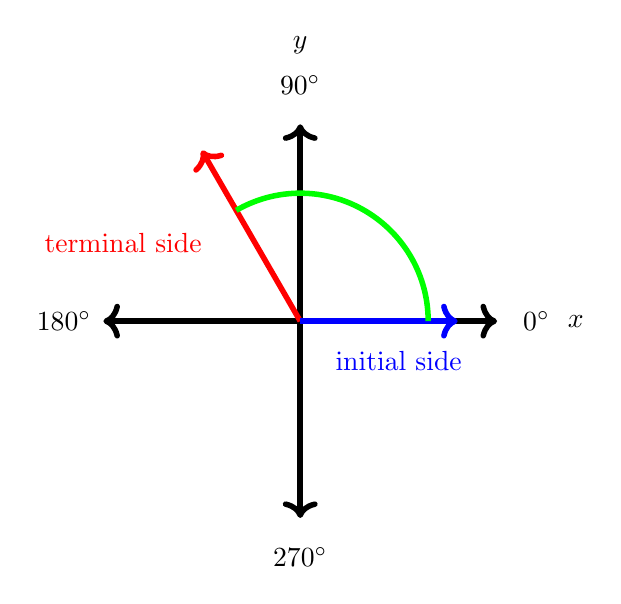
\begin{tikzpicture}[scale=2.5]
	
	
	\coordinate (a) at (0,1);
	\coordinate (b) at (0,-1);
	\coordinate (c) at (-1,0);
	\coordinate (d) at (1,0);
	\coordinate (e) at (0,0);
	\coordinate (f) at (-.5,.866);
	\draw[line width=2pt, <->](a) -- (b);
	\draw[line width=2pt, <->](c) -- (d);
	\draw[red, line width=2pt, ->] (e) -- (f);
	\draw[blue, line width=2pt, ->] (e) -- (.8,0);
	\draw[green, line width=2pt](.65,0)arc[radius=.65, start angle=0, end angle= 120];
	\node at (0,1.4) {$y$};
	\node at (0,1.2) {$90^\circ$};
	\node at (1.4,0) {$x$};
	\node at (1.2,0) {$0^\circ$};
	\node at (-1.2,0) {$180^\circ$};
	\node at (0,-1.2) {$270^\circ$};
	\node[blue] at (.5,-.2) {initial side};
	\node[red] at (-.9,.4) {terminal side};

	
	\end{tikzpicture}
\end{center}

This is called \textbf{Standard Position} of an angle.\\

\pagebreak

\subsection*{Standard Position}

\begin{multicols}{2}

\textbf{Example 1) } Approximate the angle\\

\vspace{12pt}

	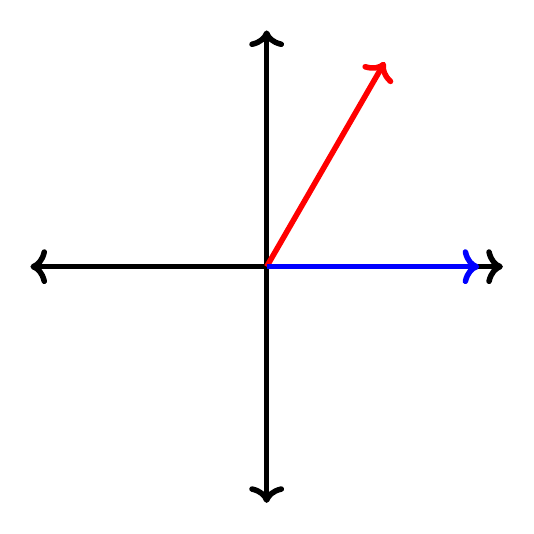
\begin{tikzpicture}[scale=3]
	
	
	\coordinate (a) at (0,1);
	\coordinate (b) at (0,-1);
	\coordinate (c) at (-1,0);
	\coordinate (d) at (1,0);
	\coordinate (e) at (0,0);
	\coordinate (f) at (.5,0.866);
	
	\draw[line width=2pt, <->] (a) -- (b);
	\draw[line width=2pt, <->] (c) -- (d);
	\draw[red, line width=2pt, ->] (e) -- (f);
	\draw[blue, line width=2pt, ->] (0,0) -- (.9,0);
	
	
	\end{tikzpicture}

\columnbreak

\textbf{Example 2)} Draw a $210^\circ$ angle\\

\vspace{12pt}

	\begin{tikzpicture}[scale=3]
	
	
	\coordinate (a) at (0,1);
	\coordinate (b) at (0,-1);
	\coordinate (c) at (-1,0);
	\coordinate (d) at (1,0);

	
	\draw[line width=2pt, <->] (a) -- (b);
	\draw[line width=2pt, <->] (c) -- (d);
	
	\end{tikzpicture}
\end{multicols}

\vspace{32pt}

\textbf{You Try:}

\begin{multicols}{2}

Approximate the angle\\

\vspace{12pt}

	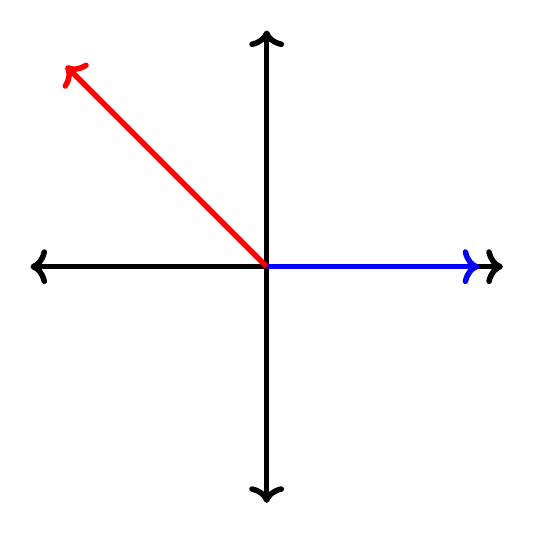
\begin{tikzpicture}[scale=3]
	
	
	\coordinate (a) at (0,1);
	\coordinate (b) at (0,-1);
	\coordinate (c) at (-1,0);
	\coordinate (d) at (1,0);
	\coordinate (e) at (0,0);
	\coordinate (f) at (-.85,0.85);
	
	\draw[line width=2pt, <->] (a) -- (b);
	\draw[line width=2pt, <->] (c) -- (d);
	\draw[red, line width=2pt,->] (e) -- (f);
	\draw[blue, line width=2pt, ->] (0,0) -- (.9,0);
	
	
	\end{tikzpicture}

\columnbreak

Draw a $100^\circ$ angle.\\

\vspace{12pt}

	\begin{tikzpicture}[scale=3]
	
	
	\coordinate (a) at (0,1);
	\coordinate (b) at (0,-1);
	\coordinate (c) at (-1,0);
	\coordinate (d) at (1,0);

	
	\draw[line width=2pt, <->] (a) -- (b);
	\draw[line width=2pt, <->] (c) -- (d);
	
	\end{tikzpicture}
\end{multicols}

\pagebreak

\subsection*{Negative Angles}

A negative angle will go \textit{clockwise} instead of \textit{counter-clockwise}\\

\begin{multicols}{2}

\textbf{Example 3)} Approximate the angle\\

\vspace{12pt}

	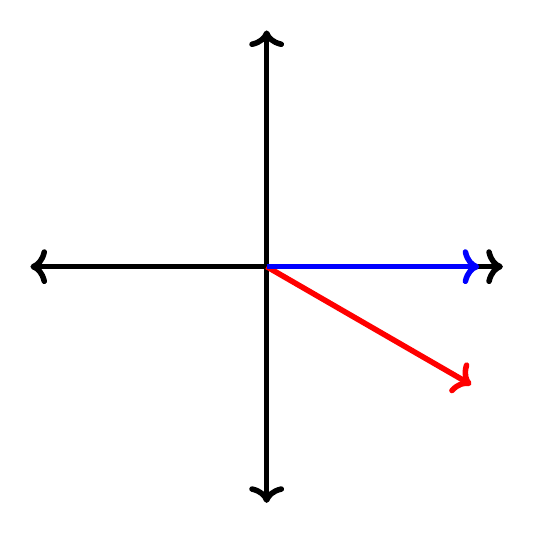
\begin{tikzpicture}[scale=3]
	
	
	\coordinate (a) at (0,1);
	\coordinate (b) at (0,-1);
	\coordinate (c) at (-1,0);
	\coordinate (d) at (1,0);
	\coordinate (e) at (0,0);
	\coordinate (f) at (.866,-0.5);
	
	\draw[line width=2pt, <->] (a) -- (b);
	\draw[line width=2pt, <->] (c) -- (d);
	\draw[red,line width=2pt,->] (e) -- (f);
	\draw[blue, line width=2pt, ->] (0,0) -- (.9,0);
		
	
	\end{tikzpicture}

\columnbreak

\textbf{Example 4)} Draw a $-100^\circ$ angle;

\vspace{12pt}

	\begin{tikzpicture}[scale=3]
	
	
	\coordinate (a) at (0,1);
	\coordinate (b) at (0,-1);
	\coordinate (c) at (-1,0);
	\coordinate (d) at (1,0);

	
	\draw[line width=2pt, <->] (a) -- (b);
	\draw[line width=2pt, <->] (c) -- (d);
	
	\end{tikzpicture}
\end{multicols}

\vspace{32pt}

\textbf{You Try:}

\begin{multicols}{2}

Approximate the angle\\

\vspace{12pt}

	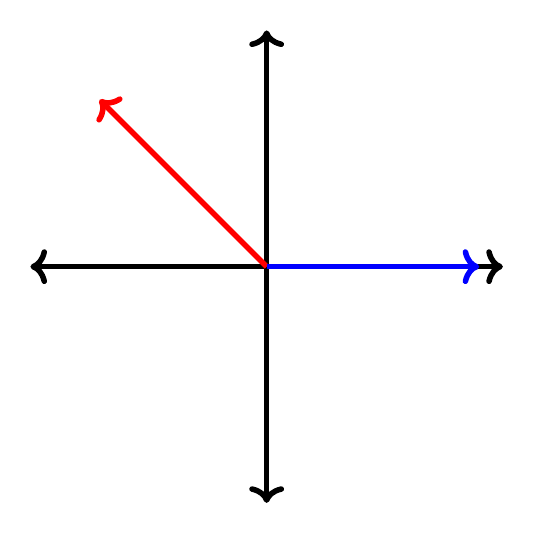
\begin{tikzpicture}[scale=3]
	
	
	\coordinate (a) at (0,1);
	\coordinate (b) at (0,-1);
	\coordinate (c) at (-1,0);
	\coordinate (d) at (1,0);
	\coordinate (e) at (0,0);
	\coordinate (f) at (-.707,0.707);
	
	\draw[line width=2pt, <->] (a) -- (b);
	\draw[line width=2pt, <->] (c) -- (d);
	\draw[red,line width=2pt,->] (e) -- (f);
	\draw[blue, line width=2pt, ->] (0,0) -- (.9,0);
	
	
	\end{tikzpicture}

\columnbreak

Draw a $-80^\circ$ angle\\

\vspace{12pt}

	\begin{tikzpicture}[scale=3]
	
	
	\coordinate (a) at (0,1);
	\coordinate (b) at (0,-1);
	\coordinate (c) at (-1,0);
	\coordinate (d) at (1,0);

	
	\draw[line width=2pt, <->] (a) -- (b);
	\draw[line width=2pt, <->] (c) -- (d);
	
	\end{tikzpicture}
\end{multicols}


\pagebreak

\subsection*{Co-Terminal Angles}

Two angles with the same terminal side are called \textbf{co-terminal angles}. ($0^\circ = 360^\circ$ or $90^\circ=-270^\circ$)\\

\begin{multicols}{2}

\textbf{Example 5)} Two ways to write the angle.\\

\vspace{12pt}

	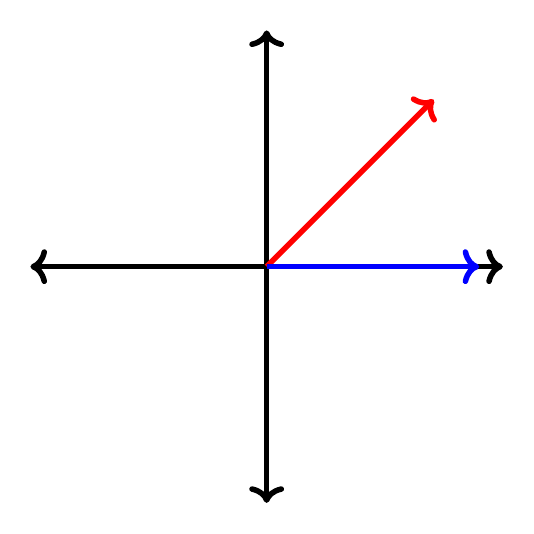
\begin{tikzpicture}[scale=3]
	
	
	\coordinate (a) at (0,1);
	\coordinate (b) at (0,-1);
	\coordinate (c) at (-1,0);
	\coordinate (d) at (1,0);
	\coordinate (e) at (0,0);
	\coordinate (f) at (.707,0.707);
	
	\draw[line width=2pt, <->] (a) -- (b);
	\draw[line width=2pt, <->] (c) -- (d);
	\draw[red,line width=2pt,->] (e) -- (f);
	\draw[blue, line width=2pt, ->] (0,0) -- (.9,0);
	
	
	\end{tikzpicture}

\columnbreak

\textbf{Example 6)} What is coterminal to $210^\circ$?\\

\vspace{12pt}

	\begin{tikzpicture}[scale=3]
	
	
	\coordinate (a) at (0,1);
	\coordinate (b) at (0,-1);
	\coordinate (c) at (-1,0);
	\coordinate (d) at (1,0);

	
	\draw[line width=2pt, <->] (a) -- (b);
	\draw[line width=2pt, <->] (c) -- (d);
	
	\end{tikzpicture}
\end{multicols}

\vspace{32pt}

\textbf{You Try:}\\

\begin{multicols}{2}

Two ways to write the angle.\\

\vspace{12pt}

	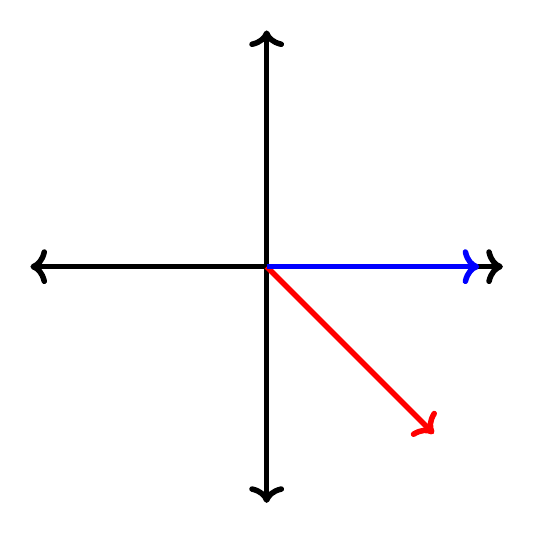
\begin{tikzpicture}[scale=3]
	
	
	\coordinate (a) at (0,1);
	\coordinate (b) at (0,-1);
	\coordinate (c) at (-1,0);
	\coordinate (d) at (1,0);
	\coordinate (e) at (0,0);
	\coordinate (f) at (.707,-0.707);
	
	\draw[line width=2pt, <->] (a) -- (b);
	\draw[line width=2pt, <->] (c) -- (d);
	\draw[red,line width=2pt,->] (e) -- (f);
	\draw[blue, line width=2pt, ->] (0,0) -- (.9,0);
	
	
	\end{tikzpicture}

\columnbreak

What is coterminal to $500^\circ$?\\

\vspace{12pt}

	\begin{tikzpicture}[scale=3]
	
	
	\coordinate (a) at (0,1);
	\coordinate (b) at (0,-1);
	\coordinate (c) at (-1,0);
	\coordinate (d) at (1,0);

	
	\draw[line width=2pt, <->] (a) -- (b);
	\draw[line width=2pt, <->] (c) -- (d);
	
	\end{tikzpicture}
\end{multicols}

\section*{Radians}

There are two main ways to measure angles. The first one that you know is called \textit{degree angle measure}. The new type that we're learning is called \textit{radian angle measure} (which is what ''rad'' stands for on your calculator).\\

The circumference of a circle is $2\pi r$. So a circle with a radius of $1$ has a circumference of $2\pi$.

$$360^\circ = 2\pi  \text{ radians} \hspace{1in} \pi \text{ radians}=180^\circ$$

\begin{center}
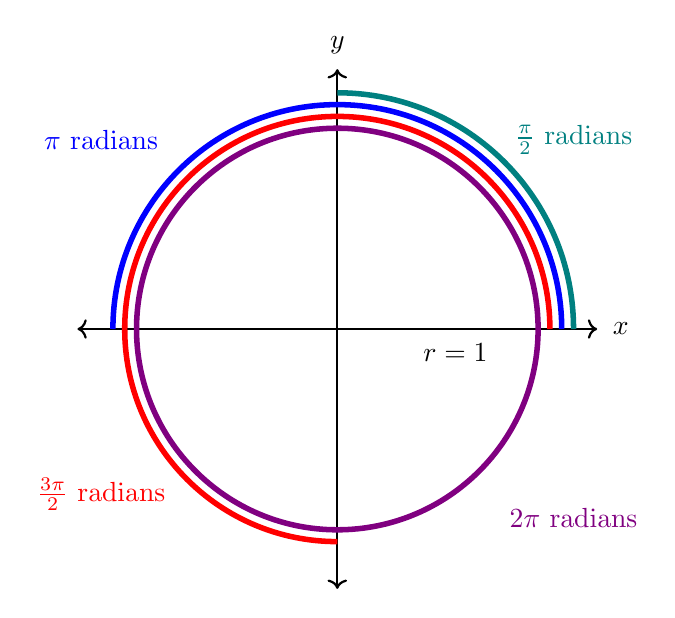
\begin{tikzpicture}[scale=3]


%	\draw[thick] (0,0)circle[radius=.9];
	\draw[thick, <->] (1.1,0) -- (-1.1,0);
	\draw[thick, <->] (0,1.1) -- (0,-1.1);
	\node at (1.2,0) {$x$};
	\node at (0,1.2){$y$};
	\node at (.5,-.1){$r=1$};
	\draw[line width=2pt,teal](1,0) arc [radius=1,start angle=0,end angle=90];
	\draw[line width=2pt,blue] (.95,0) arc [radius=.95,start angle=0, end angle=180];
	\draw[line width=2pt,red] (.9,0) arc[radius=.9,start angle=0, end angle=270];
	\draw[line width=2pt,violet] circle[radius=.85];
	\node[blue] at (-1,.8){$\pi$ radians};
	\node[violet] at (1,-.8){$2\pi$ radians};
	\node[teal] at (1,.8){$\frac{\pi}{2}$ radians};
	\node[red] at (-1,-.7){$\frac{3\pi}{2}$ radians};

\end{tikzpicture}
\end{center}


To convert from degree to radian $\times \frac{\pi}{180}$\\

\vspace{12pt}

To convert from radian to degree $\times \frac{180}{\pi}$\\


\begin{multicols}{2}
\begin{enumerate}
	\setlength\itemsep{24pt}
	
	\item $190^\circ$ is how many radians?\\
	
		
	\item 2 radians is how many degrees?\\
	
	
	\item $270^\circ$ is how many radians?\\
	
		
	\item $\frac{\pi}{6}$ radians is how many degrees?\\
	
	
	\item $45^\circ$ is how many radians?\\
	
	\item $\frac{\pi}{3}$ is how many degrees?\\
	
	\item $100^\circ$ is how many radians?\\
	
	\item $\frac{3\pi}{2}$ is how many degrees?\\
		
\end{enumerate}
\end{multicols}


\section{Practice}

Draw a $\frac{3\pi}{4}$ radians\\
\begin{tikzpicture}[scale=3]
	
	
	\coordinate (a) at (0,1);
	\coordinate (b) at (0,-1);
	\coordinate (c) at (-1,0);
	\coordinate (d) at (1,0);

	
	\draw[line width=2pt, <->] (a) -- (b);
	\draw[line width=2pt, <->] (c) -- (d);
	
	\end{tikzpicture}


Draw a $-\frac{5\pi}{6}$ radians\\
\begin{tikzpicture}[scale=3]
	
	
	\coordinate (a) at (0,1);
	\coordinate (b) at (0,-1);
	\coordinate (c) at (-1,0);
	\coordinate (d) at (1,0);

	
	\draw[line width=2pt, <->] (a) -- (b);
	\draw[line width=2pt, <->] (c) -- (d);
	
	\end{tikzpicture}
	
Find the angle between $0$ and $2\pi$ that is coterminal to $-\frac{23\pi}{10}$

\section*{Tips on Radians}

\subsection*{Multiples of $90^\circ$}


\begin{multicols}{2}

$90^\circ=\frac{\pi}{2}$ radians \\

$180^\circ=\frac{2\pi}{2}$ radians $=\pi$ radians \\
 
$270^\circ=\frac{3\pi}{2}$ radians \\
 
 $360^\circ=\frac{4\pi}{2}$ radians $=2\pi$ radians\\

\end{multicols}

\subsection*{Multiples of $60^\circ$}


\begin{multicols}{2}

$60^\circ=\frac{\pi}{3}$ radians \\
 
$120^\circ=\frac{2\pi}{3}$ radians \\
  
$180^\circ=\frac{3\pi}{3}$ radians $=\pi$ radians \\
   
$240^\circ=\frac{4\pi}{3}$ radians \\
    
$300^\circ=\frac{5\pi}{3}$ radians \\
     
$360^\circ=\frac{6\pi}{3}$ radians $=2\pi$ radians \\

\end{multicols}

\subsection*{Multiples of $45^\circ$}


\begin{multicols}{2}
$45^\circ=\frac{\pi}{4}$ radians \\

$90^\circ=\frac{2\pi}{4}$ radians $=\frac{\pi}{2}$ radians \\

$135^\circ=\frac{3\pi}{4}$ radians \\

$180^\circ=\frac{4\pi}{4}$ radians $=\pi$ radians \\

$225^\circ=\frac{5\pi}{4}$ radians \\

$270^\circ=\frac{6\pi}{4}$ radians $=\frac{3\pi}{2}$ radians \\

$315^\circ=\frac{7\pi}{4}$ radians \\

$360^\circ=\frac{8\pi}{4}$ radians $=2\pi$ radians \\
\end{multicols}

\subsection*{Multiples of $30^\circ$}

\begin{multicols}{2}

$30^\circ=\frac{\pi}{6}$ radians \\

$30^\circ=\frac{2\pi}{6}$ radians $=\frac{\pi}{3}$ radians \\

$90^\circ=\frac{3\pi}{6}$ radians $=\frac{\pi}{2}$ radians \\
 
$120^\circ=\frac{4\pi}{6}$ radians $=\frac{2\pi}{3}$ radians \\

$150^\circ=\frac{5\pi}{6}$ radians \\
  
$180^\circ=\frac{6\pi}{6}$ radians $=\pi$ radians \\

$210^\circ=\frac{7\pi}{6}$ radians \\
   
$240^\circ=\frac{8\pi}{6}$ radians $=\frac{4\pi}{3}$ radians \\

$270^\circ=\frac{9\pi}{6}$ radians $=\frac{3\pi}{2}$ radians \\
    
$300^\circ=\frac{10\pi}{6}$ radians $=\frac{5\pi}{3}$ radians \\

 $330^\circ=\frac{11\pi}{6}$ radians\\
     
$360^\circ=\frac{12\pi}{6}$ radians $=2\pi$ radians \\

\end{multicols}

\section*{Evaluating Trig Functions of Any Angle \\ Extending the Trig Ratios}

\begin{center}
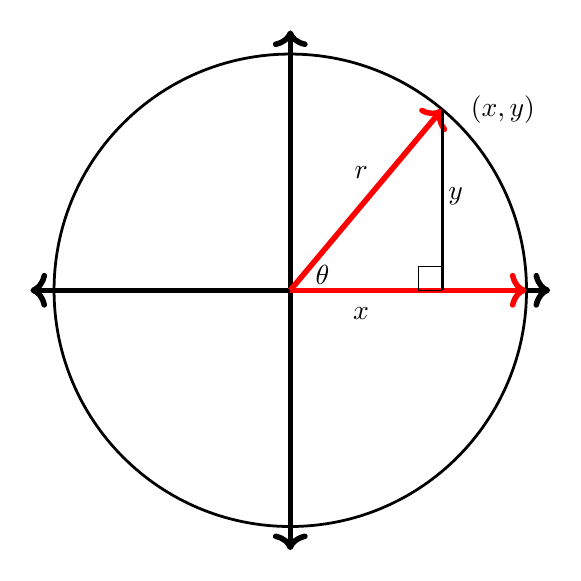
\begin{tikzpicture}[scale=3]

	\draw[line width=1pt] (0,0) circle[radius=1];
	\draw[line width=2pt,<->] (0,1.1) -- (0,-1.1);
	\draw[line width=2pt,<->] (1.1,0) -- (-1.1,0);
	\draw[red, line width=2pt,->] (0,0) -- (1,0);
	\draw[red,line width=2pt, ->] (0,0) -- (0.64278761,0.766044443);
	\draw[line width=1pt] (0.64278761,0.766044443) -- (0.64278761,0);
%	\draw[fill](0.64278761,0.766044443)circle[radius=.04];
	\node at (.9,0.76604443){$(x,y)$};
	\node at (.3,.5){$r$};
	\node at (.3,-.1){$x$};
	\node at (.7,.4){$y$};
	
	\coordinate (a) at (1,0);
	\coordinate (b) at (0,0);
	\coordinate (c) at (0,1);
	\coordinate (d) at (0.64278761,0.766044443);
	\coordinate (e) at (0.64278761,0);
	\tkzMarkRightAngle[size=.1](b,e,d)
	\tkzLabelAngle[pos=.15](a,b,d){$\theta$}

\end{tikzpicture}
\end{center}

$$\sin(\theta)=\frac{y}{r}$$

$$\cos(\theta)=\frac{x}{r}$$

$$\tan(\theta)=\frac{y}{x}$$

\hrulefill

Use the Pythagorean Theorem to find $r$, $r=$\\

\begin{multicols}{2}

\begin{center}
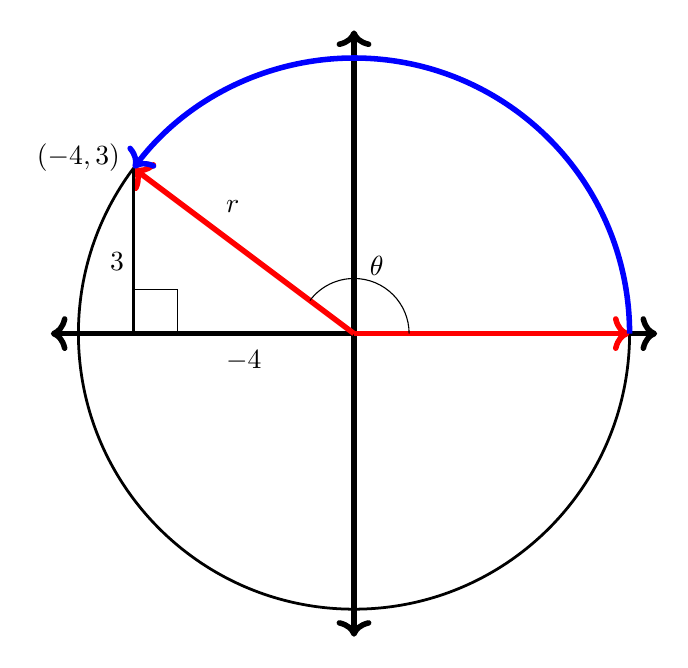
\begin{tikzpicture}[scale=.7]

	\draw[line width=1pt] (0,0) circle[radius=5];
	\draw[line width=2pt,<->] (0,5.5) -- (0,-5.5); %y-axis
	\draw[line width=2pt,<->] (5.5,0) -- (-5.5,0); %x-axis
	\draw[red, line width=2pt,->] (0,0) -- (5,0); %initial side
	\draw[red,line width=2pt, ->] (0,0) -- (-4,3); %terminal side
	\draw[line width=1pt] (-4,3) -- (-4,0);
	\node at (-5,3.2){$(-4,3)$};
	\node at (-2.2,2.3){$r$};
	\node at (-2,-.5){$-4$};
	\node at (-4.3,1.3){$3$};

	\draw[line width=2pt,blue,->] (5,0) arc[radius=5,start angle=0, end angle=143.1301024];
	
	
	\coordinate (a) at (5,0);
	\coordinate (b) at (0,0);
	\coordinate (c) at (0,5);
	\coordinate (d) at (-4,3);
	\coordinate (e) at (-4,0);
	\tkzMarkRightAngle[size=.8](b,e,d)
	\tkzLabelAngle[pos=1.3](a,b,d){$\theta$}
	\tkzMarkAngle(a,b,d)

\end{tikzpicture}
\end{center}
\columnbreak

$$x=-4 , y=3, r=5$$

$$\sin(\theta)=\frac{\hspace{.5cm}}{}$$

$$\cos(\theta)=\frac{\hspace{.5cm}}{}$$

$$\tan(\theta)=\frac{\hspace{.5cm}}{}$$

\end{multicols}

\pagebreak

Use the Pythagorean Theorem to find $r$, $r=$\\

\begin{multicols}{2}

\begin{center} %Make this one Quadrant 3
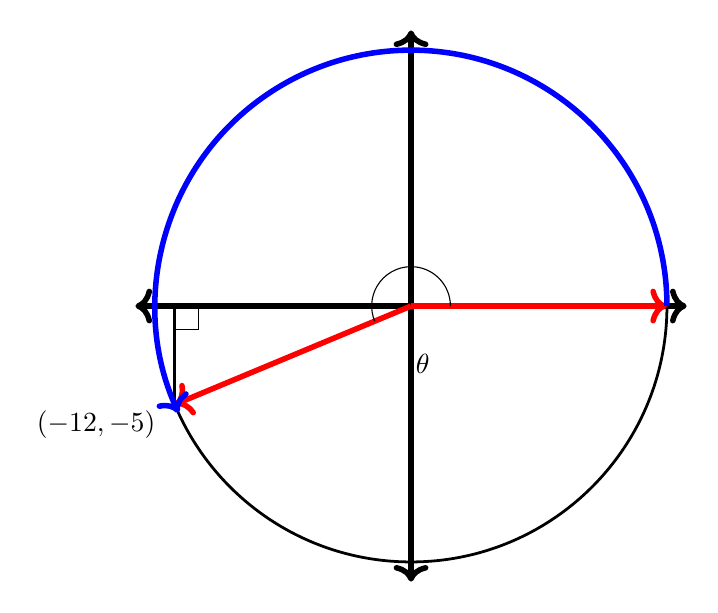
\begin{tikzpicture}[scale=.25]

	\draw[line width=1pt] (0,0) circle[radius=13];
	\draw[line width=2pt,<->] (0,14) -- (0,-14); %y-axis
	\draw[line width=2pt,<->] (14,0) -- (-14,0); %x-axis
	\draw[red, line width=2pt,->] (0,0) -- (13,0); %initial side
	\draw[red,line width=2pt, ->] (0,0) -- (-12,-5); %terminal side
	\draw[line width=1pt] (-12,-5) -- (-12,0);
	\node at (-16,-6){$(-12,-5)$};
	\draw[line width=2pt,blue,->] (13,0) arc[radius=13,start angle=0, end angle=204.6243184];

	\coordinate (a) at (5,0);
	\coordinate (b) at (0,0);
	\coordinate (c) at (0,5);
	\coordinate (d) at (-12,-5);
	\coordinate (e) at (-12,0);
	\tkzMarkRightAngle[size=1.2](b,e,d)
	\tkzLabelAngle[pos=-3](a,b,d){$\theta$}
	\tkzMarkAngle[size=2](a,b,d)

\end{tikzpicture}
\end{center}
\columnbreak

$$x=\underline{\hspace{1cm}} , y=\underline{\hspace{1cm}}, r=\underline{\hspace{1cm}}$$

$$\sin(\theta)=\frac{y}{r}=$$

$$\cos(\theta)=\frac{x}{r}=$$

$$\tan(\theta)=\frac{y}{x}=$$

$$\theta = ?$$
\end{multicols}

\hrulefill

Use the Pythagorean Theorem to find $r$, $r=$\\

\begin{multicols}{2} %Make this one Quadrant 4

\begin{center}
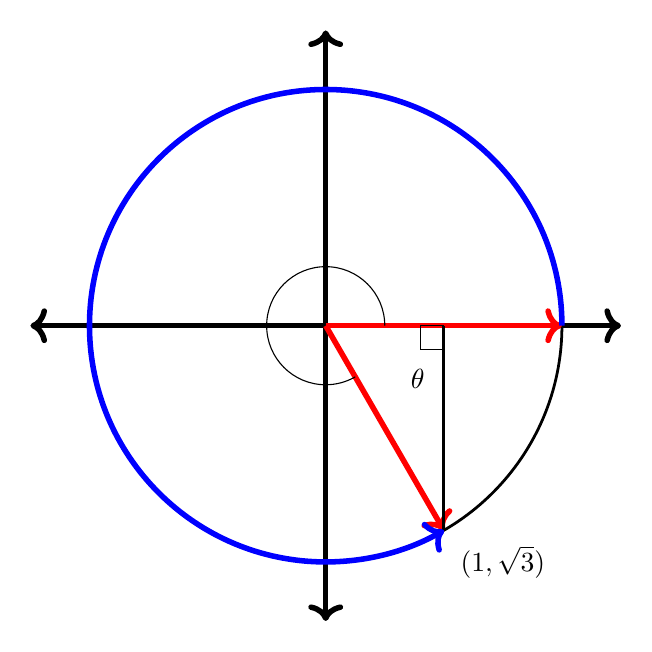
\begin{tikzpicture}[scale=1.5]

	\draw[line width=1pt] (0,0) circle[radius=2];
	\draw[line width=2pt,<->] (0,2.5) -- (0,-2.5); %y-axis
	\draw[line width=2pt,<->] (2.5,0) -- (-2.5,0); %x-axis
	\draw[red, line width=2pt,->] (0,0) -- (2,0); %initial side
	\draw[red,line width=2pt, ->] (0,0) -- (1,-1.732050808); %terminal side
	\draw[line width=1pt] (1,-1.732050808) -- (1,0);
	\node at (1.5,-2){$(1,\sqrt{3})$};
	
	\draw[line width=2pt,blue,->] (2,0) arc[radius=2,start angle=0, end angle=300];
	
	\coordinate (a) at (2,0);
	\coordinate (b) at (0,0);
	\coordinate (c) at (0,2);
	\coordinate (d) at (1,-1.732050808);
	\coordinate (e) at (1,0);
	\tkzMarkRightAngle[size=.2](b,e,d)
	\tkzLabelAngle[pos=-.9](a,b,d){$\theta$}
	\tkzMarkAngle[size=.5](a,b,d)

\end{tikzpicture}
\end{center}
\columnbreak

$$x=\underline{\hspace{1cm}} , y=\underline{\hspace{1cm}}, r=\underline{\hspace{1cm}}$$

$$\sin(\theta)=$$

$$\cos(\theta)=$$

$$\tan(\theta)=$$



\end{multicols}

\section*{The Unit Circle}

The unit circle is a circle whose radius is 1 and has a center about the origin. The values of $\sin(\theta)$ and $\cos(\theta)$ are just the $y$-values and $x$-values respectively. \\

%$$(\cos\theta,\sin\theta)$$

% based on http://www.texample.net/tikz/examples/unit-circle/
%
    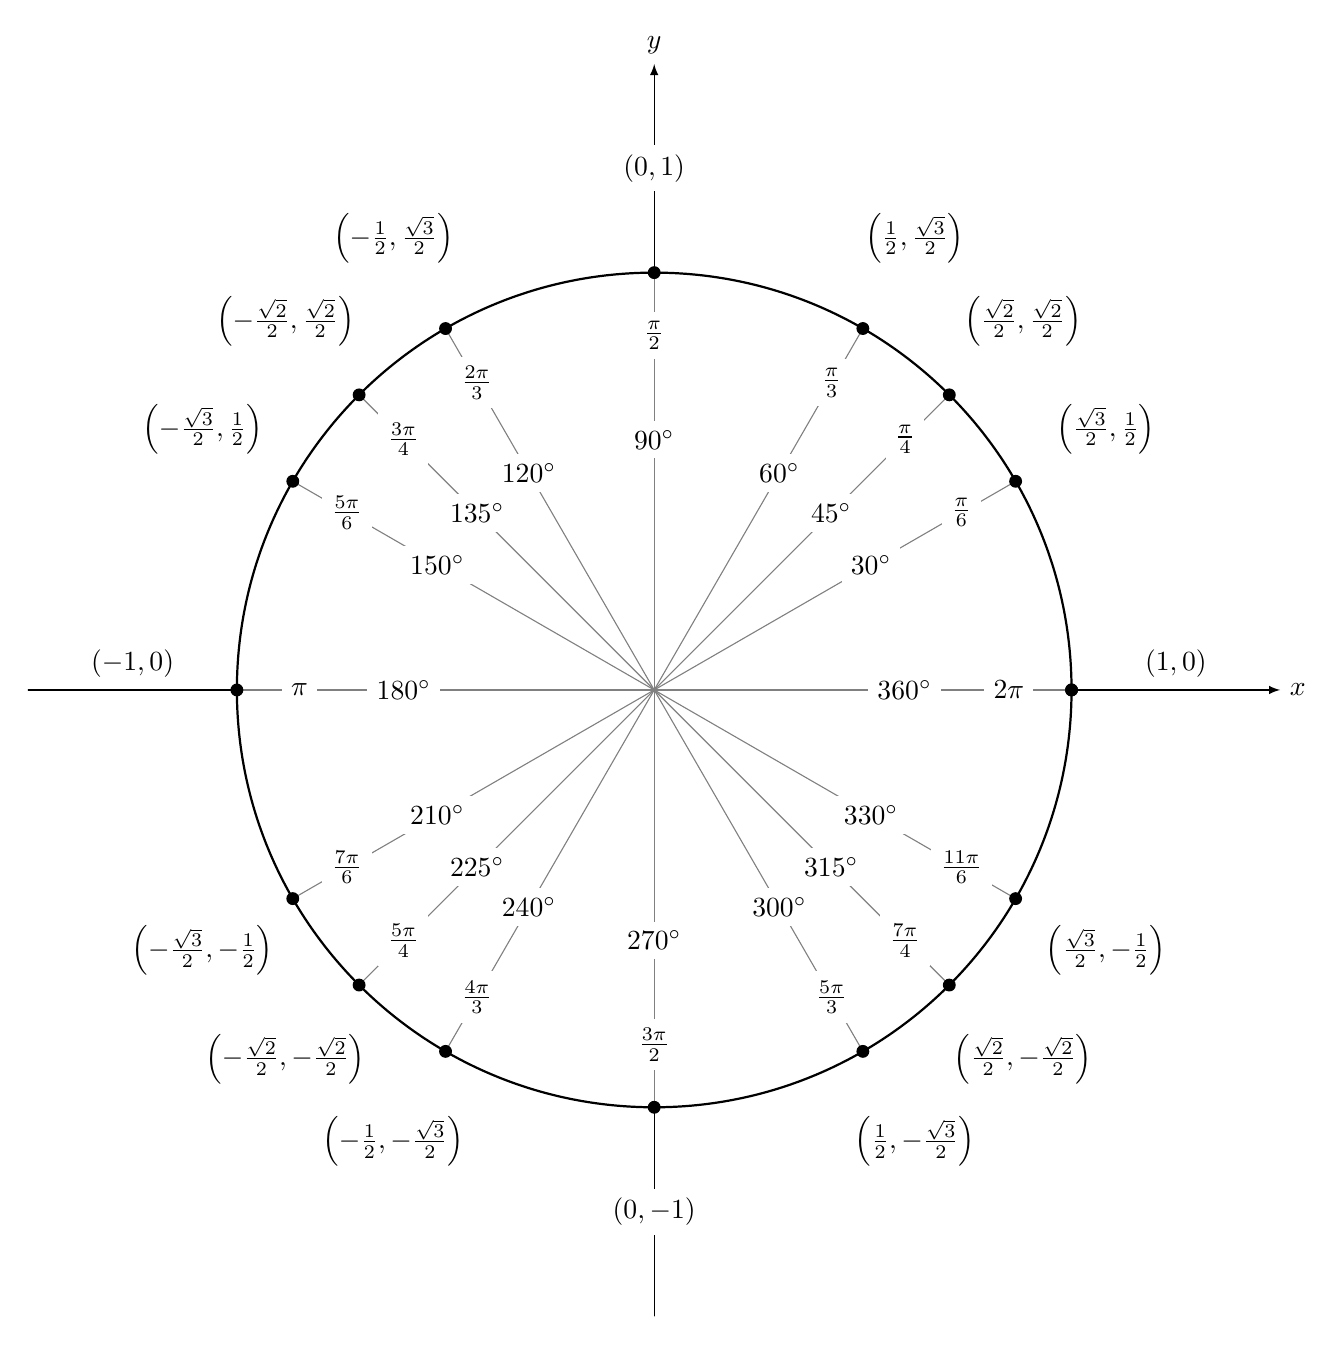
\begin{tikzpicture}[scale=5.3,cap=round,>=latex]
        % draw the coordinates
        \draw[->] (-1.5cm,0cm) -- (1.5cm,0cm) node[right,fill=white] {$x$};
        \draw[->] (0cm,-1.5cm) -- (0cm,1.5cm) node[above,fill=white] {$y$};

        % draw the unit circle
        \draw[thick] (0cm,0cm) circle(1cm);

        \foreach \x in {0,30,...,360} {
                % lines from center to point
                \draw[gray] (0cm,0cm) -- (\x:1cm);
                % dots at each point
                \filldraw[black] (\x:1cm) circle(0.4pt);
                % draw each angle in degrees
                \draw (\x:0.6cm) node[fill=white] {$\x^\circ$};
        }

		\foreach \x in {45,135,225,315}{
				\draw[gray](0cm,0cm) -- (\x:1cm);
				\filldraw[black] (\x:1cm) circle(0.4pt);
				\draw (\x:0.6cm) node[fill=white] {$\x^\circ$};
		}

        % draw each angle in radians
        \foreach \x/\xtext in {
            30/\frac{\pi}{6},
            45/\frac{\pi}{4},
            60/\frac{\pi}{3},
            90/\frac{\pi}{2},
            120/\frac{2\pi}{3},
            135/\frac{3\pi}{4},
            150/\frac{5\pi}{6},
            180/\pi,
            210/\frac{7\pi}{6},
            225/\frac{5\pi}{4},
            240/\frac{4\pi}{3},
            270/\frac{3\pi}{2},
            300/\frac{5\pi}{3},
            315/\frac{7\pi}{4},
            330/\frac{11\pi}{6},
            360/2\pi}
                \draw (\x:0.85cm) node[fill=white] {$\xtext$};

        \foreach \x/\xtext/\y in {
            % the coordinates for the first quadrant
            30/\frac{\sqrt{3}}{2}/\frac{1}{2},
            45/\frac{\sqrt{2}}{2}/\frac{\sqrt{2}}{2},
            60/\frac{1}{2}/\frac{\sqrt{3}}{2},
            % the coordinates for the second quadrant
            150/-\frac{\sqrt{3}}{2}/\frac{1}{2},
            135/-\frac{\sqrt{2}}{2}/\frac{\sqrt{2}}{2},
            120/-\frac{1}{2}/\frac{\sqrt{3}}{2},
            % the coordinates for the third quadrant
            210/-\frac{\sqrt{3}}{2}/-\frac{1}{2},
            225/-\frac{\sqrt{2}}{2}/-\frac{\sqrt{2}}{2},
            240/-\frac{1}{2}/-\frac{\sqrt{3}}{2},
            % the coordinates for the fourth quadrant
            330/\frac{\sqrt{3}}{2}/-\frac{1}{2},
            315/\frac{\sqrt{2}}{2}/-\frac{\sqrt{2}}{2},
            300/\frac{1}{2}/-\frac{\sqrt{3}}{2}}
                \draw (\x:1.25cm) node[fill=white] {$\left(\xtext,\y\right)$};

        % draw the horizontal and vertical coordinates
        % the placement is better this way
        \draw (-1.25cm,0cm) node[above=1pt] {$(-1,0)$}
              (1.25cm,0cm)  node[above=1pt] {$(1,0)$}
              (0cm,-1.25cm) node[fill=white] {$(0,-1)$}
              (0cm,1.25cm)  node[fill=white] {$(0,1)$};
    \end{tikzpicture}

\section*{Reference Angles}

Reference help us remember certain trig values. As can been seen from the unit circle, the points on the circle are the same all around except for the negative signs. Basically, knowing the first quadrant values will you to know all of the angles.\\

\subsection*{Quadratal Angles}

These are angles whose terminal sides are on the axis, multiples of $90^\circ$ or $\frac{\pi}{2}$.\\

\subsection*{Reference Agnles}

\begin{center}
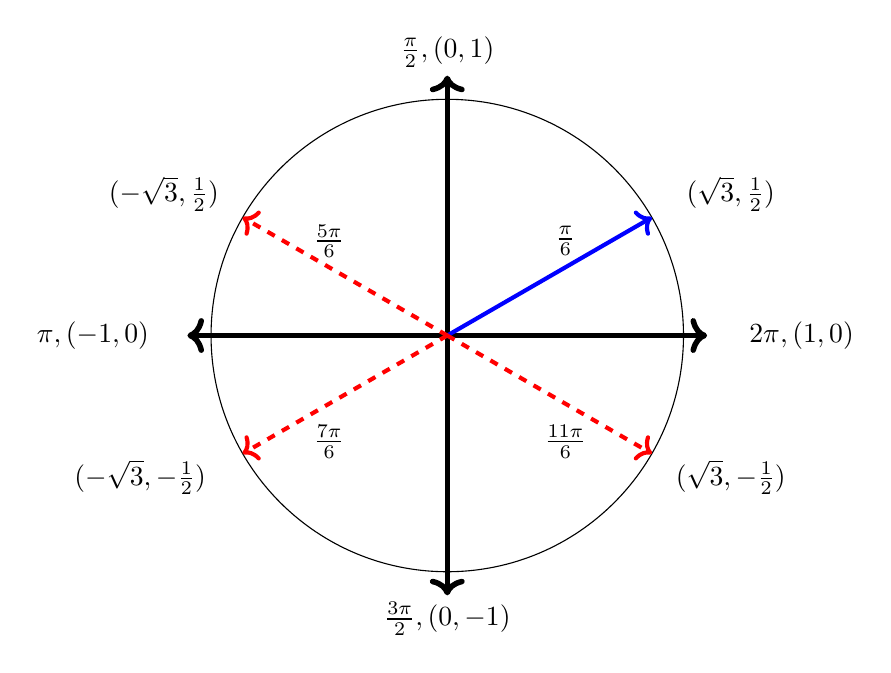
\begin{tikzpicture}[scale=3]

	\draw[line width=2pt,<->](1.1,0)--(-1.1,0);
	\draw[line width=2pt,<->](0,1.1)--(0,-1.1);
	\draw(0,0)circle[radius=1];
	\node at (0,1.2){$\frac{\pi}{2},(0,1)$};
	\node at (0,-1.2){$\frac{3\pi}{2},(0,-1)$};
	\node at (-1.5,0){$\pi,(-1,0)$};
	\node at (1.5,0){$2\pi,(1,0)$};
	\draw[blue, line width=1.5pt,->](0,0)--(0.866025404,0.5); %30 degree angle
		\draw[red,dashed, line width=1.5pt,->](0,0)--(-0.866025404,0.5); %reference angle q2
		\draw[red,dashed, line width=1.5pt,->](0,0)--(0.866025404,-0.5); %reference angle q4
		\draw[red,dashed, line width=1.5pt,->](0,0)--(-0.866025404,-0.5); %reference angle q3
	
	\node at (1.2,.6){$(\sqrt{3},\frac{1}{2})$};
	\node at (-1.2,.6){$(-\sqrt{3},\frac{1}{2})$};		
	\node at (1.2,-.6){$(\sqrt{3},-\frac{1}{2})$};
	\node at (-1.3,-.6){$(-\sqrt{3},-\frac{1}{2})$};
	
	\node at (.5,.4){$\frac{\pi}{6}$};
	\node at (-.5,.4){$\frac{5\pi}{6}$};
	\node at (-.5,-.45){$\frac{7\pi}{6}$};
	\node at (.5,-.45){$\frac{11\pi}{6}$};
	
	

\end{tikzpicture}
\end{center}

The $x$ and $y$ values are the same on each of these



\bgroup
\def\arraystretch{3.3}%  1 is the default, change whatever you need
\setlength{\tabcolsep}{.4in}
\begin{tabular}{c c c c}

$\sin\frac{\pi}{6}=$ & $\sin\frac{5\pi}{6}=$ & $\sin\frac{7\pi}{6}=$ & $\sin\frac{11\pi}{6}=$ \\

$\cos\frac{\pi}{6}=$ & $\cos\frac{5\pi}{6}=$ & $\cos\frac{7\pi}{6}=$ & $\cos\frac{11\pi}{6}=$ \\

$\tan\frac{\pi}{6}=$ & $\tan\frac{5\pi}{6}=$ & $\tan\frac{7\pi}{6}=$ & $\tan\frac{11\pi}{6}=$ \\

\end{tabular}
\egroup


\section*{Unit Review}

\hfill NAME:\underline{\hspace*{3in}}

\subsection*{General Angles}

Draw each angle, name the quadrant, list one positive and one negative coterminal angle. (4 points each)\\

\begin{enumerate}
\begin{multicols}{3}
\item Draw a $210^\circ$ angle\\

\vspace{12pt}

	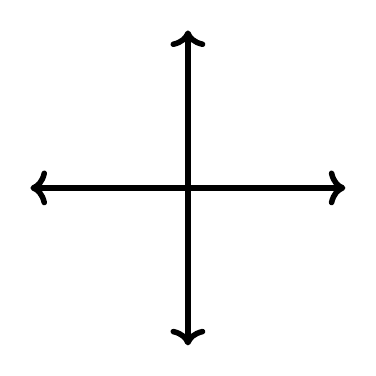
\begin{tikzpicture}[scale=2]
	
	
	\coordinate (a) at (0,1);
	\coordinate (b) at (0,-1);
	\coordinate (c) at (-1,0);
	\coordinate (d) at (1,0);

	
	\draw[line width=2pt, <->] (a) -- (b);
	\draw[line width=2pt, <->] (c) -- (d);
	
	\end{tikzpicture}

Quadrant:\underline{\hspace{1in}}\\

+ coterminal:\underline{\hspace{1in}}\\

- coterminal:\underline{\hspace{1in}}

\columnbreak

\item Draw a $66^\circ$ angle\\

\vspace{12pt}

	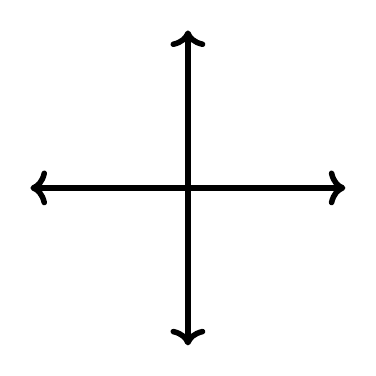
\begin{tikzpicture}[scale=2]
	
	
	\coordinate (a) at (0,1);
	\coordinate (b) at (0,-1);
	\coordinate (c) at (-1,0);
	\coordinate (d) at (1,0);

	
	\draw[line width=2pt, <->] (a) -- (b);
	\draw[line width=2pt, <->] (c) -- (d);
	
	\end{tikzpicture}

Quadrant:\underline{\hspace{1in}}\\

+ coterminal:\underline{\hspace{1in}}\\

- coterminal:\underline{\hspace{1in}}

\columnbreak

\item Draw a $345^\circ$ angle\\

\vspace{12pt}

	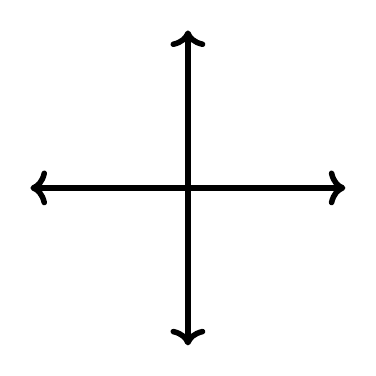
\begin{tikzpicture}[scale=2]
	
	
	\coordinate (a) at (0,1);
	\coordinate (b) at (0,-1);
	\coordinate (c) at (-1,0);
	\coordinate (d) at (1,0);

	
	\draw[line width=2pt, <->] (a) -- (b);
	\draw[line width=2pt, <->] (c) -- (d);
	
	\end{tikzpicture}

Quadrant:\underline{\hspace{1in}}\\

+ coterminal:\underline{\hspace{1in}}\\

- coterminal:\underline{\hspace{1in}}
	
\end{multicols}
\end{enumerate}

\subsection*{Radians}

Convert from radians to degrees, or from degrees to radians. (2 points each).\\

\begin{enumerate}[resume]
\begin{multicols}{2}

\item $30^\circ$\\

\item $80^\circ$\\

\item $225^\circ$\\

\item $110^\circ$\\

\item $330^\circ$\\

\columnbreak

\item $\frac{\pi}{9}$\\

\item $\frac{2\pi}{9}$\\

\item $\frac{7\pi}{4}$\\

\item $\frac{9\pi}{10}$\\

\item $\frac{3\pi}{2}$\\

\end{multicols}
\end{enumerate}


\pagebreak

\subsection*{Evaluating Trig functions}

Evaluate $\sin$, $\cos$, and $\tan$ at the given point. (4 points each)\\

\begin{center}
$\sin\theta=\frac{y}{r}$ \ $cos\theta=\frac{x}{r}$ \ $\tan\theta=\frac{y}{x}$\\
\end{center}

\vspace{12pt}

\begin{enumerate}[resume]
\begin{multicols}{2}

\item $(12,5)$, r=\underline{\hspace{.7in}}\\

$\sin\theta=$\underline{\hspace{1in}}\\

$\cos\theta=$\underline{\hspace{1in}}\\

$\tan\theta=$\underline{\hspace{1in}}\\

\item $(-6,8)$, r=\underline{\hspace{.7in}}\\

$\sin\theta=$\underline{\hspace{1in}}\\

$\cos\theta=$\underline{\hspace{1in}}\\

$\tan\theta=$\underline{\hspace{1in}}\\

\item $(-2,-2)$, r=\underline{\hspace{.7in}}\\

$\sin\theta=$\underline{\hspace{1in}}\\

$\cos\theta=$\underline{\hspace{1in}}\\

$\tan\theta=$\underline{\hspace{1in}}\\

\item $(4,-3)$, r=\underline{\hspace{.7in}}\\

$\sin\theta=$\underline{\hspace{1in}}\\

$\cos\theta=$\underline{\hspace{1in}}\\

$\tan\theta=$\underline{\hspace{1in}}\\

\end{multicols}
\end{enumerate}

\subsection*{Unit Circle \& Reference Angles}

Use your unit circle (2 points each)\\

\begin{enumerate}[resume]

\item What is the reference angle for $300^\circ$?\\

\item Name 2 angles whose reference angle is $45^\circ$\\

\item How many reference angles are there for $30^\circ$\\

\item What is the $\sin$ and $\cos$ value at $150^\circ$?\\

\end{enumerate}

\section*{Unit Test.}

\hfill NAME:\underline{\hspace*{3in}}

\subsection*{General Angles}

Draw each angle, name the quadrant, list one positive and one negative coterminal angle. (4 points each)\\

\begin{enumerate}
\begin{multicols}{3}
\item Draw a $110^\circ$ angle\\

\vspace{12pt}

	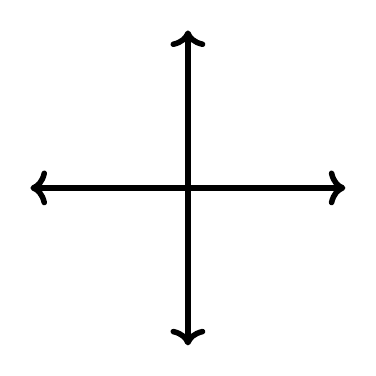
\begin{tikzpicture}[scale=2]
	
	
	\coordinate (a) at (0,1);
	\coordinate (b) at (0,-1);
	\coordinate (c) at (-1,0);
	\coordinate (d) at (1,0);

	
	\draw[line width=2pt, <->] (a) -- (b);
	\draw[line width=2pt, <->] (c) -- (d);
	
	\end{tikzpicture}

Quadrant:\underline{\hspace{1in}}\\

+ coterminal:\underline{\hspace{1in}}\\

- coterminal:\underline{\hspace{1in}}

\columnbreak

\item Draw a $-56^\circ$ angle\\

\vspace{12pt}

	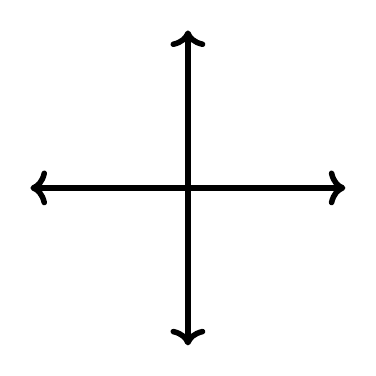
\begin{tikzpicture}[scale=2]
	
	
	\coordinate (a) at (0,1);
	\coordinate (b) at (0,-1);
	\coordinate (c) at (-1,0);
	\coordinate (d) at (1,0);

	
	\draw[line width=2pt, <->] (a) -- (b);
	\draw[line width=2pt, <->] (c) -- (d);
	
	\end{tikzpicture}

Quadrant:\underline{\hspace{1in}}\\

+ coterminal:\underline{\hspace{1in}}\\

- coterminal:\underline{\hspace{1in}}

\columnbreak

\item Draw a $45^\circ$ angle\\

\vspace{12pt}

	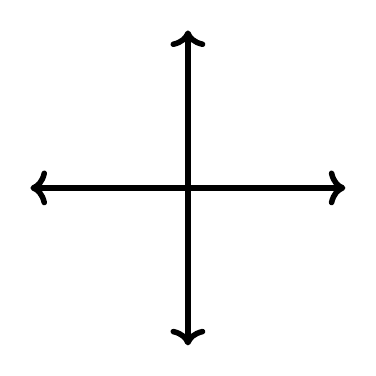
\begin{tikzpicture}[scale=2]
	
	
	\coordinate (a) at (0,1);
	\coordinate (b) at (0,-1);
	\coordinate (c) at (-1,0);
	\coordinate (d) at (1,0);

	
	\draw[line width=2pt, <->] (a) -- (b);
	\draw[line width=2pt, <->] (c) -- (d);
	
	\end{tikzpicture}

Quadrant:\underline{\hspace{1in}}\\

+ coterminal:\underline{\hspace{1in}}\\

- coterminal:\underline{\hspace{1in}}
	
\end{multicols}
\end{enumerate}

\subsection*{Radians}

Convert from radians to degrees, or from degrees to radians. (2 points each).\\

\begin{enumerate}[resume]
\begin{multicols}{2}

\item $45^\circ$\\

\item $210^\circ$\\

\item $160^\circ$\\

\item $18^\circ$\\

\item $600^\circ$\\

\columnbreak

\item $\frac{\pi}{18}$\\

\item $\frac{5\pi}{18}$\\

\item $\frac{7\pi}{9}$\\

\item $\frac{3\pi}{4}$\\

\item $\frac{\pi}{6}$\\

\end{multicols}
\end{enumerate}


\pagebreak

\subsection*{Evaluating Trig functions}

Evaluate $\sin$, $\cos$, and $\tan$ at the given point. (4 points each)\\

\begin{center}
$\sin\theta=\frac{y}{r}$ \ $cos\theta=\frac{x}{r}$ \ $\tan\theta=\frac{y}{x}$\\
\end{center}

\vspace{12pt}

\begin{enumerate}[resume]
\begin{multicols}{2}

\item $(5,-12)$, r=\underline{\hspace{.7in}}\\

$\sin\theta=$\underline{\hspace{1in}}\\

$\cos\theta=$\underline{\hspace{1in}}\\

$\tan\theta=$\underline{\hspace{1in}}\\

\item $(8,-6)$, r=\underline{\hspace{.7in}}\\

$\sin\theta=$\underline{\hspace{1in}}\\

$\cos\theta=$\underline{\hspace{1in}}\\

$\tan\theta=$\underline{\hspace{1in}}\\

\item $(1,1)$, r=\underline{\hspace{.7in}}\\

$\sin\theta=$\underline{\hspace{1in}}\\

$\cos\theta=$\underline{\hspace{1in}}\\

$\tan\theta=$\underline{\hspace{1in}}\\

\item $(-4,3)$, r=\underline{\hspace{.7in}}\\

$\sin\theta=$\underline{\hspace{1in}}\\

$\cos\theta=$\underline{\hspace{1in}}\\

$\tan\theta=$\underline{\hspace{1in}}\\

\end{multicols}
\end{enumerate}

\subsection*{Unit Circle \& Reference Angles}

Use your unit circle (2 points each)\\

\begin{enumerate}[resume]

\item What is the reference angle for $210^\circ$?\\

\item Name 2 angles whose reference angle is $30^\circ$\\

\item How many reference angles are there for $60^\circ$\\

\item What is the $\sin$ and $\cos$ value at $120^\circ$?\\

$\sin(120^\circ)=$ \hspace{1in} $\cos(120^\circ)=$

\end{enumerate}

\section*{Unit Test:}

\hfill NAME:\underline{\hspace*{3in}}

\subsection*{General Angles}

Draw each angle, name the quadrant, list one positive and one negative coterminal angle. (4 points each)\\

\begin{enumerate}
\begin{multicols}{3}
\item Draw a $70^\circ$ angle\\

\vspace{12pt}

	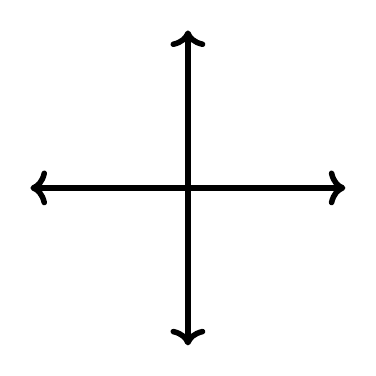
\begin{tikzpicture}[scale=2]
	
	
	\coordinate (a) at (0,1);
	\coordinate (b) at (0,-1);
	\coordinate (c) at (-1,0);
	\coordinate (d) at (1,0);

	
	\draw[line width=2pt, <->] (a) -- (b);
	\draw[line width=2pt, <->] (c) -- (d);
	
	\end{tikzpicture}

Quadrant:\underline{\hspace{1in}}\\

+ coterminal:\underline{\hspace{1in}}\\

- coterminal:\underline{\hspace{1in}}

\columnbreak

\item Draw a $190^\circ$ angle\\

\vspace{12pt}

	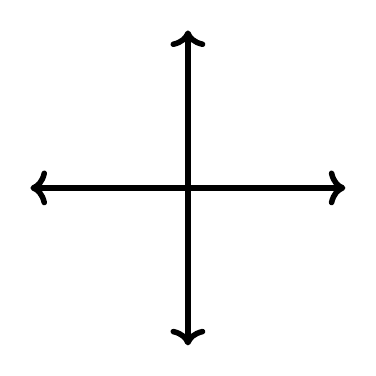
\begin{tikzpicture}[scale=2]
	
	
	\coordinate (a) at (0,1);
	\coordinate (b) at (0,-1);
	\coordinate (c) at (-1,0);
	\coordinate (d) at (1,0);

	
	\draw[line width=2pt, <->] (a) -- (b);
	\draw[line width=2pt, <->] (c) -- (d);
	
	\end{tikzpicture}

Quadrant:\underline{\hspace{1in}}\\

+ coterminal:\underline{\hspace{1in}}\\

- coterminal:\underline{\hspace{1in}}

\columnbreak

\item Draw a $315^\circ$ angle\\

\vspace{12pt}

	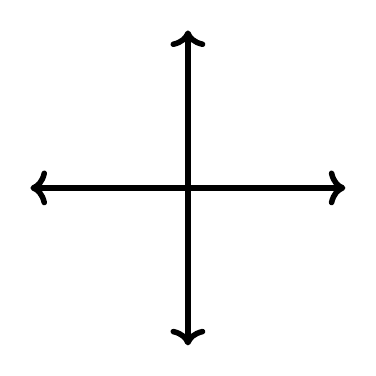
\begin{tikzpicture}[scale=2]
	
	
	\coordinate (a) at (0,1);
	\coordinate (b) at (0,-1);
	\coordinate (c) at (-1,0);
	\coordinate (d) at (1,0);

	
	\draw[line width=2pt, <->] (a) -- (b);
	\draw[line width=2pt, <->] (c) -- (d);
	
	\end{tikzpicture}

Quadrant:\underline{\hspace{1in}}\\

+ coterminal:\underline{\hspace{1in}}\\

- coterminal:\underline{\hspace{1in}}
	
\end{multicols}
\end{enumerate}

\subsection*{Radians}

Convert from radians to degrees, or from degrees to radians. (2 points each).\\

\begin{enumerate}[resume]
\begin{multicols}{2}

\item $25^\circ$\\

\item $150^\circ$\\

\item $240^\circ$\\

\item $10^\circ$\\

\item $315^\circ$\\

\columnbreak

\item $\frac{\pi}{90}$\\

\item $\frac{2\pi}{90}$\\

\item $\frac{\pi}{5}$\\

\item $\frac{2\pi}{3}$\\

\item $\frac{3\pi}{4}$\\

\end{multicols}
\end{enumerate}


\pagebreak

\subsection*{Evaluating Trig functions}

Evaluate $\sin$, $\cos$, and $\tan$ at the given point. (4 points each)\\

\begin{center}
$\sin\theta=\frac{y}{r}$ \ $cos\theta=\frac{x}{r}$ \ $\tan\theta=\frac{y}{x}$\\
\end{center}

\vspace{12pt}

\begin{enumerate}[resume]
\begin{multicols}{2}

\item $(3,4)$, r=\underline{\hspace{.7in}}\\

$\sin\theta=$\underline{\hspace{1in}}\\

$\cos\theta=$\underline{\hspace{1in}}\\

$\tan\theta=$\underline{\hspace{1in}}\\

\item $(-8,6)$, r=\underline{\hspace{.7in}}\\

$\sin\theta=$\underline{\hspace{1in}}\\

$\cos\theta=$\underline{\hspace{1in}}\\

$\tan\theta=$\underline{\hspace{1in}}\\

\item $(-1,-1)$, r=\underline{\hspace{.7in}}\\

$\sin\theta=$\underline{\hspace{1in}}\\

$\cos\theta=$\underline{\hspace{1in}}\\

$\tan\theta=$\underline{\hspace{1in}}\\

\item $(-7,24)$, r=\underline{\hspace{.7in}}\\

$\sin\theta=$\underline{\hspace{1in}}\\

$\cos\theta=$\underline{\hspace{1in}}\\

$\tan\theta=$\underline{\hspace{1in}}\\

\end{multicols}
\end{enumerate}

\subsection*{Unit Circle \& Reference Angles}

Use your unit circle (2 points each)\\

\begin{enumerate}[resume]

\item What is the reference angle for $330^\circ$?\\

\item Name 2 angles whose reference angle is $30^\circ$\\

\item How many reference angles are there for $60^\circ$\\

\item What is the $\sin$ and $\cos$ value at $240^\circ$?\\

$\sin(240^\circ)=$ \hspace{1in} $\cos(240^\circ)=$

\end{enumerate}

\section*{Unit Test::}

\hfill NAME:\underline{\hspace*{3in}}

\subsection*{General Angles}

Draw each angle, name the quadrant, list one positive and one negative coterminal angle. (4 points each)\\

\begin{enumerate}
\begin{multicols}{3}
\item Draw a $100^\circ$ angle\\

\vspace{12pt}

	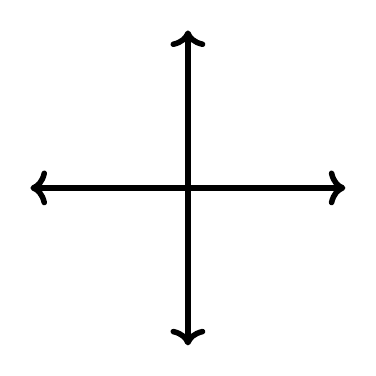
\begin{tikzpicture}[scale=2]
	
	
	\coordinate (a) at (0,1);
	\coordinate (b) at (0,-1);
	\coordinate (c) at (-1,0);
	\coordinate (d) at (1,0);

	
	\draw[line width=2pt, <->] (a) -- (b);
	\draw[line width=2pt, <->] (c) -- (d);
	
	\end{tikzpicture}

Quadrant:\underline{\hspace{1in}}\\

+ coterminal:\underline{\hspace{1in}}\\

- coterminal:\underline{\hspace{1in}}

\columnbreak

\item Draw a $200^\circ$ angle\\

\vspace{12pt}

	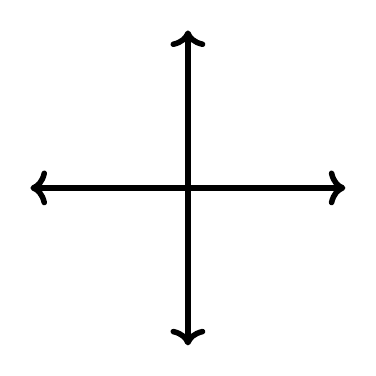
\begin{tikzpicture}[scale=2]
	
	
	\coordinate (a) at (0,1);
	\coordinate (b) at (0,-1);
	\coordinate (c) at (-1,0);
	\coordinate (d) at (1,0);

	
	\draw[line width=2pt, <->] (a) -- (b);
	\draw[line width=2pt, <->] (c) -- (d);
	
	\end{tikzpicture}

Quadrant:\underline{\hspace{1in}}\\

+ coterminal:\underline{\hspace{1in}}\\

- coterminal:\underline{\hspace{1in}}

\columnbreak

\item Draw a $300^\circ$ angle\\

\vspace{12pt}

	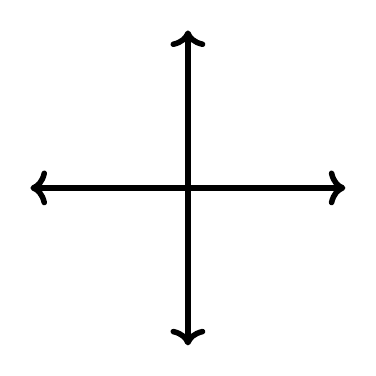
\begin{tikzpicture}[scale=2]
	
	
	\coordinate (a) at (0,1);
	\coordinate (b) at (0,-1);
	\coordinate (c) at (-1,0);
	\coordinate (d) at (1,0);

	
	\draw[line width=2pt, <->] (a) -- (b);
	\draw[line width=2pt, <->] (c) -- (d);
	
	\end{tikzpicture}

Quadrant:\underline{\hspace{1in}}\\

+ coterminal:\underline{\hspace{1in}}\\

- coterminal:\underline{\hspace{1in}}
	
\end{multicols}
\end{enumerate}

\subsection*{Radians}

Convert from radians to degrees, or from degrees to radians. (2 points each).\\

\begin{enumerate}[resume]
\begin{multicols}{2}

\item $100^\circ$\\

\item $150^\circ$\\

\item $200^\circ$\\

\item $250^\circ$\\

\item $300^\circ$\\

\columnbreak

\item $\frac{\pi}{10}$\\

\item $\frac{\pi}{5}$\\

\item $\frac{5\pi}{4}$\\

\item $\frac{7\pi}{3}$\\

\item $\frac{3\pi}{5}$\\

\end{multicols}
\end{enumerate}


\pagebreak

\subsection*{Evaluating Trig functions}

Evaluate $\sin$, $\cos$, and $\tan$ at the given point. (4 points each)\\

\begin{center}
$\sin\theta=\frac{y}{r}$ \ $cos\theta=\frac{x}{r}$ \ $\tan\theta=\frac{y}{x}$\\
\end{center}

\vspace{12pt}

\begin{enumerate}[resume]
\begin{multicols}{2}

\item $(24,7)$, r=\underline{\hspace{.7in}}\\

$\sin\theta=$\underline{\hspace{1in}}\\

$\cos\theta=$\underline{\hspace{1in}}\\

$\tan\theta=$\underline{\hspace{1in}}\\

\item $(-5,12)$, r=\underline{\hspace{.7in}}\\

$\sin\theta=$\underline{\hspace{1in}}\\

$\cos\theta=$\underline{\hspace{1in}}\\

$\tan\theta=$\underline{\hspace{1in}}\\

\item $(-3,3)$, r=\underline{\hspace{.7in}}\\

$\sin\theta=$\underline{\hspace{1in}}\\

$\cos\theta=$\underline{\hspace{1in}}\\

$\tan\theta=$\underline{\hspace{1in}}\\

\item $(-3,4)$, r=\underline{\hspace{.7in}}\\

$\sin\theta=$\underline{\hspace{1in}}\\

$\cos\theta=$\underline{\hspace{1in}}\\

$\tan\theta=$\underline{\hspace{1in}}\\

\end{multicols}
\end{enumerate}

\subsection*{Unit Circle \& Reference Angles}

Use your unit circle (2 points each)\\

\begin{enumerate}[resume]

\item What is the reference angle for $135^\circ$?\\

\item Name 2 angles whose reference angle is $30^\circ$\\

\item How many reference angles are there for $45^\circ$\\

\item What is the $\sin$ and $\cos$ value at $210^\circ$?\\

$\sin(210^\circ)=$ \hspace{1in} $\cos(210^\circ)=$

\end{enumerate}

\section*{Unit Test}

\hfill NAME:\underline{\hspace*{3in}}

\subsection*{General Angles}

Draw each angle, name the quadrant, list one positive and one negative coterminal angle. (4 points each)\\

\begin{enumerate}
\begin{multicols}{3}
\item Draw a $10^\circ$ angle\\

\vspace{12pt}

	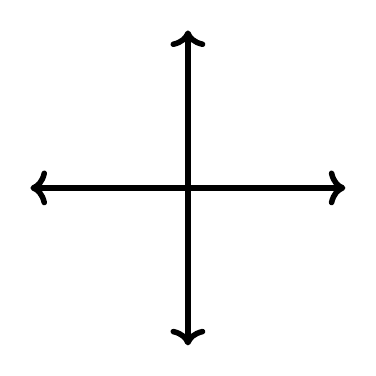
\begin{tikzpicture}[scale=2]
	
	
	\coordinate (a) at (0,1);
	\coordinate (b) at (0,-1);
	\coordinate (c) at (-1,0);
	\coordinate (d) at (1,0);

	
	\draw[line width=2pt, <->] (a) -- (b);
	\draw[line width=2pt, <->] (c) -- (d);
	
	\end{tikzpicture}

Quadrant:\underline{\hspace{1in}}\\

+ coterminal:\underline{\hspace{1in}}\\

- coterminal:\underline{\hspace{1in}}

\columnbreak

\item Draw a $100^\circ$ angle\\

\vspace{12pt}

	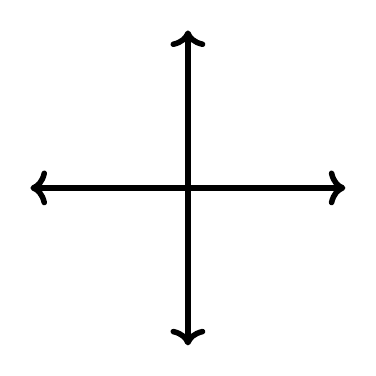
\begin{tikzpicture}[scale=2]
	
	
	\coordinate (a) at (0,1);
	\coordinate (b) at (0,-1);
	\coordinate (c) at (-1,0);
	\coordinate (d) at (1,0);

	
	\draw[line width=2pt, <->] (a) -- (b);
	\draw[line width=2pt, <->] (c) -- (d);
	
	\end{tikzpicture}

Quadrant:\underline{\hspace{1in}}\\

+ coterminal:\underline{\hspace{1in}}\\

- coterminal:\underline{\hspace{1in}}

\columnbreak

\item Draw a $177^\circ$ angle\\

\vspace{12pt}

	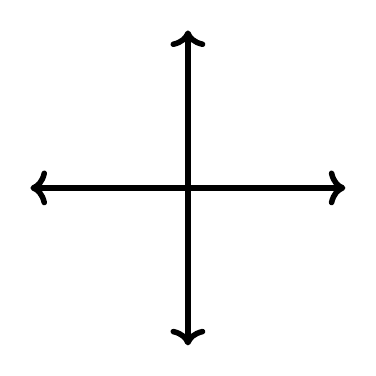
\begin{tikzpicture}[scale=2]
	
	
	\coordinate (a) at (0,1);
	\coordinate (b) at (0,-1);
	\coordinate (c) at (-1,0);
	\coordinate (d) at (1,0);

	
	\draw[line width=2pt, <->] (a) -- (b);
	\draw[line width=2pt, <->] (c) -- (d);
	
	\end{tikzpicture}

Quadrant:\underline{\hspace{1in}}\\

+ coterminal:\underline{\hspace{1in}}\\

- coterminal:\underline{\hspace{1in}}
	
\end{multicols}
\end{enumerate}

\subsection*{Radians}

Convert from radians to degrees, or from degrees to radians. (2 points each).\\

\begin{enumerate}[resume]
\begin{multicols}{2}

\item $30^\circ$\\

\item $60^\circ$\\

\item $90^\circ$\\

\item $120^\circ$\\

\item $81^\circ$\\

\columnbreak

\item $\frac{\pi}{3}$\\

\item $\frac{2\pi}{3}$\\

\item $\frac{3\pi}{2}$\\

\item $\frac{\pi}{30}$\\

\item $\frac{6\pi}{5}$\\

\end{multicols}
\end{enumerate}


\pagebreak

\subsection*{Evaluating Trig functions}

Evaluate $\sin$, $\cos$, and $\tan$ at the given point. (4 points each)\\

\begin{center}
$\sin\theta=\frac{y}{r}$ \ $cos\theta=\frac{x}{r}$ \ $\tan\theta=\frac{y}{x}$\\
\end{center}

\vspace{12pt}

\begin{enumerate}[resume]
\begin{multicols}{2}

\item $(-5,5)$, r=\underline{\hspace{.7in}}\\

$\sin\theta=$\underline{\hspace{1in}}\\

$\cos\theta=$\underline{\hspace{1in}}\\

$\tan\theta=$\underline{\hspace{1in}}\\

\item $(6,-8)$, r=\underline{\hspace{.7in}}\\

$\sin\theta=$\underline{\hspace{1in}}\\

$\cos\theta=$\underline{\hspace{1in}}\\

$\tan\theta=$\underline{\hspace{1in}}\\

\item $(-3,-4)$, r=\underline{\hspace{.7in}}\\

$\sin\theta=$\underline{\hspace{1in}}\\

$\cos\theta=$\underline{\hspace{1in}}\\

$\tan\theta=$\underline{\hspace{1in}}\\

\item $(24,7)$, r=\underline{\hspace{.7in}}\\

$\sin\theta=$\underline{\hspace{1in}}\\

$\cos\theta=$\underline{\hspace{1in}}\\

$\tan\theta=$\underline{\hspace{1in}}\\

\end{multicols}
\end{enumerate}

\subsection*{Unit Circle \& Reference Angles}

Use your unit circle (2 points each)\\

\begin{enumerate}[resume]

\item What is the reference angle for $225^\circ$?\\

\item Name 2 angles whose reference angle is $30^\circ$\\

\item How many reference angles are there for $60^\circ$\\

\item What is the $\sin$ and $\cos$ value at $180^\circ$?\\

$\sin(180)=$ \hspace{1in} $\cos(180)=$

\end{enumerate}

\section*{Graphing Trig Functions}

\pyc{2^5}

%check this out http://gma.math.ufl.edu/files/tikz.pdf

%\begin{tikzpicture}
%	\begin{axis}[my style, xtick={-3,-2,...,3}, ytick={-3,-2,...,3},
%	xmin=-3, xmax=3, ymin=-3, ymax=3]
%	\end{axis}
%\end{tikzpicture}


$y = a \sin(b x + c) + d$\\

$a=$ amplitude\\
$b=$ period (horizontal strech/compression)\\
$c=$ phase (horizontal) shift\\
$d=$ vertical shift\\


period = $\dfrac{2\pi}{b}$\\

phase shift = $-\dfrac{c}{b}$

\end{document}